\documentclass{article}
\usepackage{amsmath}
\usepackage{graphicx}
\usepackage[margin=2cm, bindingoffset=1cm, inner=2cm]{geometry}
\usepackage{hyperref}
\usepackage{textcomp}
\usepackage{float}
\usepackage{amsmath}
\usepackage{listings}
\usepackage{color}

\definecolor{dkgreen}{rgb}{0,0.6,0}
\definecolor{gray}{rgb}{0.5,0.5,0.5}
\definecolor{mauve}{rgb}{0.58,0,0.82}

\lstset{frame=tb,
   language=Java,
   aboveskip=3mm,
   belowskip=3mm,
   showstringspaces=false,
   columns=flexible,
   basicstyle={\small\ttfamily},
   numbers=none,
   numberstyle=\tiny\color{gray},
   keywordstyle=\color{blue},
   commentstyle=\color{dkgreen},
   stringstyle=\color{mauve},
   breaklines=true,
   breakatwhitespace=true
   tabsize=3
   }

\title{\bf Step-by-step Simulation Guide}
\author{Sakina Rehman}

\begin{document}
\maketitle

\begin{enumerate}

\item  \textbf{Start OOF2}. After changing into your local directory, run OOF2.

\item  \textbf{Prepare files, load module and create microstructure} First, load OOF2 with module load OOF2. Next create your own local directory for your work, and load the binary image into the working directory. Import the binary image using the code below. The microstructure will now contain your uploaded image. From the dropdown Windows menu in the OOF2 viewer, select Graphics and click New to see the uploaded microstructure.

\lstset{language=Python}
\begin{lstlisting}
 OOF.Microstructure.Create_From_ImageFile(filename='/home/nanohub/srehman6/data/results/1643665/
 grain.png', microstructure_name='grain.png', height=automatic, width=automatic)
 OOF.Windows.Graphics.New()
\end{lstlisting}

\item  \textbf{Pixel Selection and Pixel Groups}. We shall now inform OOF2 that we have two separate materials, by forming “Pixel Groups”. Using the code below, a certain colour can be selected which can be assigned to a pixel group and is named the 'black region.' The same is done for the 'white region', where the white regions in the microstructure are assigned to a pixel group.

\lstset{language=Python}
\begin{lstlisting}
OOF.Graphics_1.Toolbox.Pixel_Select.Color(source='grain.png:grain.png', range=DeltaRGB(delta_red=0,delta_green=0,delta_blue=0), points=[Point(24.7711111111,12.6462222222)], shift=0, ctrl=0)
OOF.PixelGroup.New(name='black_region', microstructure='grain.png')
OOF.PixelGroup.AddSelection(microstructure='grain.png', group='black_region')
OOF.Graphics_1.Toolbox.Pixel_Select.Color(source='grain.png:grain.png', range=DeltaRGB(delta_red=0,delta_green=0,delta_blue=0), points=[Point(55.2386666667,92.824)], shift=0, ctrl=0)
OOF.PixelGroup.New(name='white_region', microstructure='grain.png')
OOF.PixelGroup.AddSelection(microstructure='grain.png', group='white_region')
\end{lstlisting}

\item \textbf{Creating Materials}. Two materials will be created for the black and white regions of the microstructure as seen below:

\lstset{language=Python}
\begin{lstlisting}
OOF.Material.New(name='white_region', material_type='bulk')
OOF.Material.New(name='black_region', material_type='bulk')
\end{lstlisting}

The material parameters assigned to each of the materials include the Young's Modulus, Poisson ratio, thermal conductivity and thermal expansion as seen in the script below for the black region:

\lstset{language=Python}
\begin{lstlisting}
OF.Property.Copy(property='Color', new_name='colour_black_region')
OOF.Property.Parametrize.Color.colour_black_region(color=Gray(value=0.0))
OOF.Material.Add_property(name='black_region', property='Color:colour_black_region')
OOF.Property.Copy(property='Mechanical:Elasticity:Isotropic', new_name='youngs_black_region')
OOF.Property.Parametrize.Mechanical.Elasticity.Isotropic.youngs_black_region(cijkl=
IsotropicRank4TensorEnu(young=500000000000.0,poisson=0.33))
OOF.Material.Add_property(name='black_region', property='Mechanical:Elasticity:Isotropic:youngs_black_region')
OOF.Property.Copy(property='Thermal:Conductivity:Isotropic', new_name='k_black_region')
OOF.Property.Parametrize.Thermal.Conductivity.Isotropic.k_black_region(kappa=500)
OOF.Material.Add_property(name='black_region', property='Thermal:Conductivity:Isotropic:k_black_region')
OOF.Property.Copy(property='Couplings:ThermalExpansion:Isotropic', new_name='a_black_region')
OOF.Property.Parametrize.Couplings.ThermalExpansion.Isotropic.a_black_region(alpha=1000, T0=0.0)
OOF.Material.Add_property(name='black_region', property='Couplings:ThermalExpansion:Isotropic:a_black_region')
OOF.Material.Remove_property(name='black_region', property='Couplings:ThermalExpansion:Isotropic:a_black_region')
OOF.Property.Parametrize.Couplings.ThermalExpansion.Isotropic.a_black_region(alpha=5e-05, T0=0.0)
OOF.Material.Add_property(name='black_region', property='Couplings:ThermalExpansion:Isotropic:a_black_region')
\end{lstlisting}

And for the white region:

\lstset{language=Python}
\begin{lstlisting}
OOF.Property.Copy(property='Color', new_name='colour_white_region')
OOF.Property.Parametrize.Color.colour_white_region(color=Gray(value=1.0))
OOF.Material.Add_property(name='white_region', property='Color:colour_white_region')
OOF.Property.Copy(property='Mechanical:Elasticity:Isotropic', new_name='youngs_white_region')
OOF.Property.Parametrize.Mechanical.Elasticity.Isotropic.youngs_white_region(cijkl=
IsotropicRank4TensorEnu(young=100000000000.0,poisson=0.3))
OOF.Material.Add_property(name='white_region', property='Mechanical:Elasticity:Isotropic:youngs_white_region')
OOF.Property.Copy(property='Thermal:Conductivity:Isotropic', new_name='k_white_region')
OOF.Property.Parametrize.Thermal.Conductivity.Isotropic.k_white_region(kappa=100)
OOF.Material.Add_property(name='white_region', property='Thermal:Conductivity:Isotropic:k_white_region')
OOF.Property.Copy(property='Couplings:ThermalExpansion:Isotropic', new_name='a_white_region')
OOF.Property.Parametrize.Couplings.ThermalExpansion.Isotropic.a_white_region(alpha=1e-05, T0=0.0)
OOF.Material.Add_property(name='white_region', property='Couplings:ThermalExpansion:Isotropic:a_white_region')
\end{lstlisting}

The material properties for the black region and the white region are then assigned to the appropriate pixel groups using the following Python script:

\lstset{language=Python}
\begin{lstlisting}
OOF.Material.Assign(material='black_region', microstructure='grain.png', pixels='black_region')
OOF.Material.Assign(material='white_region', microstructure='grain.png', pixels='white_region')
\end{lstlisting}

\item \textbf{Creating Microstructure Skeleton.} A skeleton is created for the microstructure using a 30 by 30 QuadSkeleton grid. To improve upon the homogeneity index, the skeleton is annealed, the edges are swapped and the skeleton is smoothened. These refinement methods increase the homogeneity index to ~0.99. The code for this step is seen below:

\lstset{language=Python}
\begin{lstlisting}
OOF.Skeleton.New(name='skeleton', microstructure='grain.png', x_elements=30, y_elements=30, skeleton_geometry=QuadSkeleton(left_right_periodicity=False,top_bottom_periodicity=False))
OOF.Skeleton.Modify(skeleton='grain.png:skeleton', modifier=Anneal(targets=AllNodes(),criterion=AverageEnergy(alpha=0.9),T=0.0,delta=1.0,iteration=
FixedIteration(iterations=50)))
OOF.Skeleton.Modify(skeleton='grain.png:skeleton', modifier=SwapEdges(targets=AllElements(),criterion=AverageEnergy(alpha=0.9)))
\end{lstlisting}

\item \textbf{Generate Mesh.} From this skeleton, the FE mesh can be created. The mapping and interpolation orders will remain 1 in this case to save on computation times. The mesh is created with the following script:

\lstset{language=Python}
\begin{lstlisting}
OOF.Mesh.New(name='mesh', skeleton='grain.png:skeleton', element_types=['D2_2', 'T3_3', 'Q4_4'])
\end{lstlisting}

\item \textbf{Specify Fields and Equations.} For temperature, all fields (defined, active and in-plane) will be defined. For now, displacements/voltages shall be ignored but may be introduced. For this example we are only considering heat diffusion, so the 'Heat Eqn' shall be used. The force, stress, coloumb etc. equations shall be ignored in this simulation. This is all achieved using the following script:

\lstset{language=Python}
\begin{lstlisting}
OOF.Subproblem.Field.Define(subproblem='grain.png:skeleton:mesh:default', field=Temperature)
OOF.Subproblem.Field.Activate(subproblem='grain.png:skeleton:mesh:default', field=Temperature)
OOF.Mesh.Field.In_Plane(mesh='grain.png:skeleton:mesh', field=Temperature)
OOF.Subproblem.Equation.Activate(subproblem='grain.png:skeleton:mesh:default', equation=Heat_Eqn)
\end{lstlisting}

\item \textbf{Specify Boundary Conditions.} For this simulation, we will allow the heat to diffuse from the left hand side of the microstructure (starting at 0 C) to the right hand side (at 600C). These boundary conditions are defined in the code below:

\lstset{language=Python}
\begin{lstlisting}
OOF.Mesh.Boundary_Conditions.New(name='bc', mesh='grain.png:skeleton:mesh', condition=DirichletBC(field=Temperature,field_component='',equation=Heat_Eqn,eqn_component='',
profile=ConstantProfile(value=0.0),boundary='left'))
OOF.Mesh.Boundary_Conditions.New(name='bc<2>', mesh='grain.png:skeleton:mesh', condition=DirichletBC(field=Temperature,field_component='',equation=Heat_Eqn,eqn_component='',
profile=ConstantProfile(value=600.0),boundary='right'))
\end{lstlisting}

\item \textbf{Solver.} The tolerance is set to 1e-13 with 1000 iterations. This can be altered to what the user sees fit. To specify the solver options the following code is used:

\lstset{language=Python}
\begin{lstlisting}
OOF.Subproblem.Set_Solver(subproblem='grain.png:skeleton:mesh:default', solver_mode=BasicSolverMode(time_stepper=BasicStaticDriver(),matrix_method=
BasicIterative(tolerance=1e-13,max_iterations=1000)))
OOF.Mesh.Set_Field_Initializer(mesh='grain.png:skeleton:mesh', field=Temperature, initializer=ConstScalarFieldInit(value=0.1))
OOF.Mesh.Solve(mesh='grain.png:skeleton:mesh', endtime=0.0)
\end{lstlisting}

\item \textbf{Visualise Results.} The above code is sufficient to run the simulation using OOF2 for simple heat diffusion. However, to visualise the results a filled contour display can be added to the script as follows:

\lstset{language=Python}
\begin{lstlisting}
OOF.LayerEditor.LayerSet.Edit(window='Graphics_1', layer_number=5)
OOF.LayerEditor.LayerSet.Add_Method(method=FilledContourDisplay(when=latest,what=
getOutput('Field:Component',component='',field=Temperature),where=getOutput('original'),
min=automatic,max=automatic,levels=11,nbins=5,colormap=ThermalMap()))
OOF.LayerEditor.LayerSet.Send(window='Graphics_1')
\end{lstlisting}

For simple grain diffusion, the results are displayed below with the filled contour map:

\begin{figure}[htbp]
   \centering
   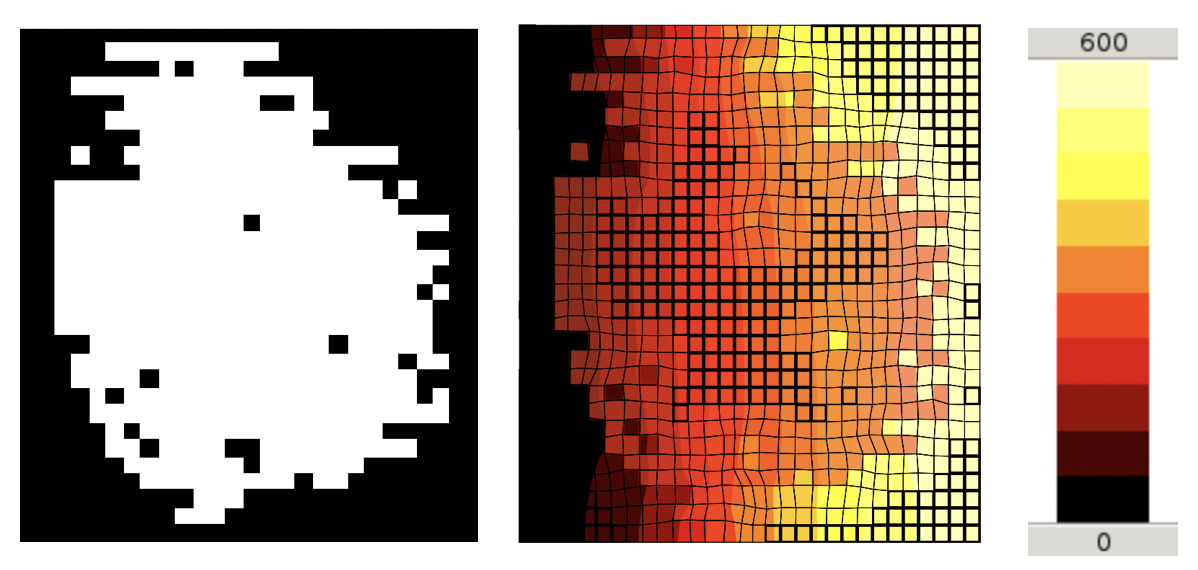
\includegraphics[width=6in]{Figures/grain_heat_diffusion} 
   \caption{Heat diffusion across a single grain}
   \label{fig:model}
\end{figure}

\end{enumerate}


\end{document}
